\documentclass{article}
\usepackage{graphicx}
\usepackage{pgfplots}
\graphicspath{ {images/} } 
\title{Learn LaTeX in 30 minutes}
\begin{document}

\maketitle

\tableofcontents

\begin{abstract}
This is a simple paragraph at the beginning of the 
document. A brief introduction about the main subject.
\end{abstract}
\newpage
%\Huge
First document. This is a simple example, with no 
extra parameters or packages included.

\textbf{Bold text Here \emph{emph Here}}

\textit{Italics text Here}

\emph{emph text Here}

\underline{underline text Here}

\subsection{Picture}
\includegraphics{sunny}
\subsection{Captions, labels and references}
\begin{figure}[h]
    \centering
    \includegraphics[width=0.25\textwidth]{sunny}
    \caption{a nice plot}
    \label{fig:mesh1}
\end{figure}
 
As you can see in the figure \ref{fig:sunny}, the 
function grows near 0. Also, in the page \pageref{fig:sunny} 
is the same example.

\subsection{Maths Formula}
There's a picture of a galaxy above

The mass-energy equivalence is described by the famous equation
 
\[E=mc^2 \]
 
discovered in 1905 by Albert Einstein. 
In natural units ($c = 1$), the formula expresses the identity
 
\begin{equation}
E=m
\end{equation}

\subsection{List}
\begin{itemize}
  \item The individual entries are indicated with a black dot, a so-called bullet.
  \item The text in the entries may be of any length.
\end{itemize}
\begin{enumerate}
  \item This is the first entry in our list
  \item The list numbers increase with each entry we add
\end{enumerate}

\subsection{Table}
%example1
\begin{center}
\begin{tabular}{ l c r }
 cell1 & cell2 & cell3 \\ 
 cell4 & cell5 & cell6 \\  
 cell7 & cell8 & cell9    
\end{tabular}
\end{center}

%example2
\begin{center}
\begin{tabular}{ |c|c|c| } 
 \hline
 cell1 & cell2 & cell3 \\ 
 cell4 & cell5 & cell6 \\ 
 cell7 & cell8 & cell9 \\ 
 \hline
\end{tabular}
\end{center}

%example3
\begin{center}
 \begin{tabular}{||c c c c||} 
 \hline
 Col1 & Col2 & Col2 & Col3 \\ [0.5ex] 
 \hline\hline
 1 & 6 & 87837 & 787 \\ 
 \hline
 2 & 7 & 78 & 5415 \\
 \hline
 3 & 545 & 778 & 7507 \\
 \hline
 4 & 545 & 18744 & 7560 \\
 \hline
 5 & 88 & 788 & 6344 \\ [1ex] 
 \hline
\end{tabular}
\end{center}

\subsection{Figure}
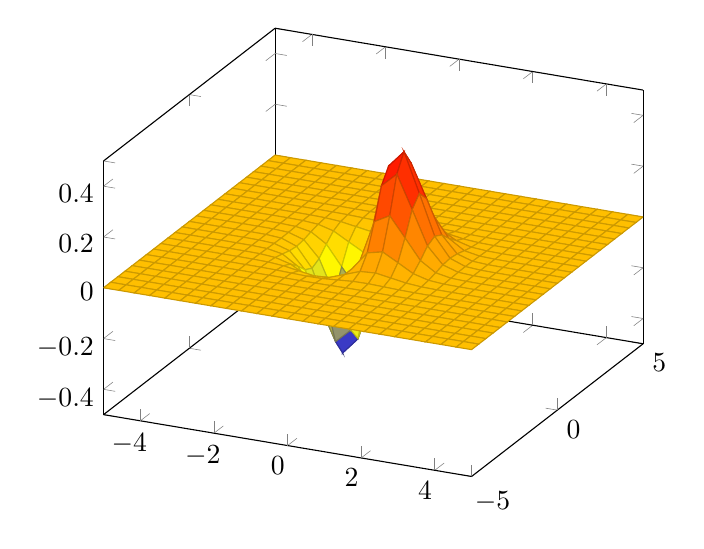
\begin{tikzpicture}
\begin{axis}
\addplot3[
    surf,
]
{exp(-x^2-y^2)*x};
%\addplot[color=red]{exp(x)};
\end{axis}
\end{tikzpicture}

\end{document}